%!TEX root = ../thesis.tex
%*******************************************************************************
%****************************** Second Chapter *********************************
%*******************************************************************************

\chapter{Imágenes}

\ifpdf
    \graphicspath{{extraimg/Figs/Raster/}{extraimg/Figs/PDF/}{extraimg/Figs/}}
\else
    \graphicspath{{extraimg/Figs/Vector/}{extraimg/Figs/}}
\fi

\begin{figure}[!htbp!]
\centering
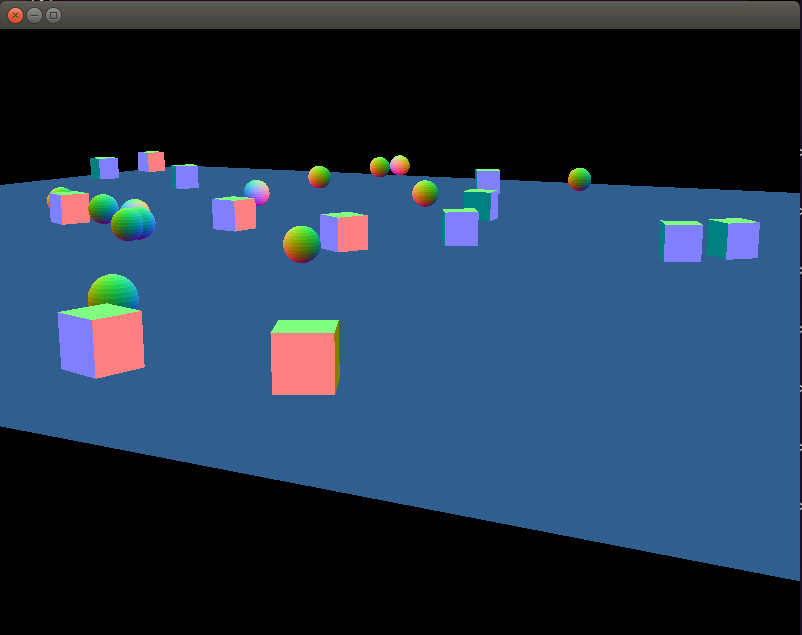
\includegraphics[width=0.5\textwidth]{test1}
\caption[Programa de prueba 1]{Juego que contiene esferas y cubos que aparecen random y se eliminan al chocar.}
\label{fig:test1}
\end{figure}

\begin{figure}[!htbp!]
\centering
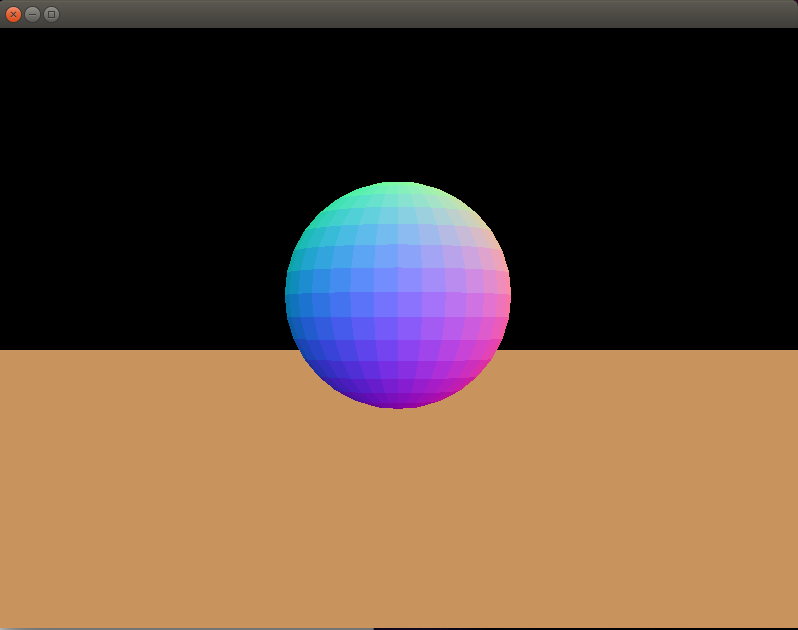
\includegraphics[width=0.5\textwidth]{test2}
\caption[Programa de prueba 2]{Juego de una pelota rebotando contra un piso.}
\label{fig:test2}
\end{figure}

\begin{figure}[!htbp!]
\centering
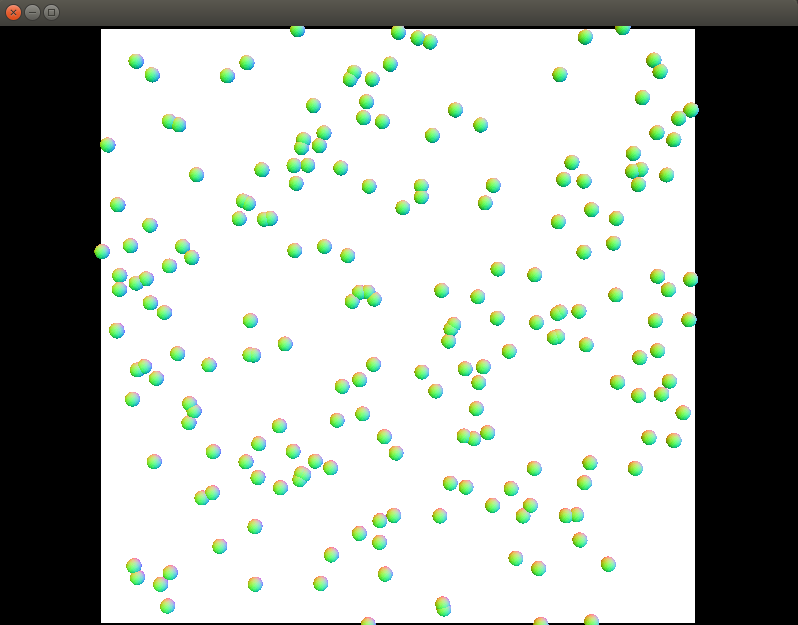
\includegraphics[width=0.5\textwidth]{test3}
\caption[Programa de prueba 3]{Juego en el que 200 esferas chocan y rebotan entre sí.}
\label{fig:test3}
\end{figure}

\begin{figure}[!htbp!]
\centering
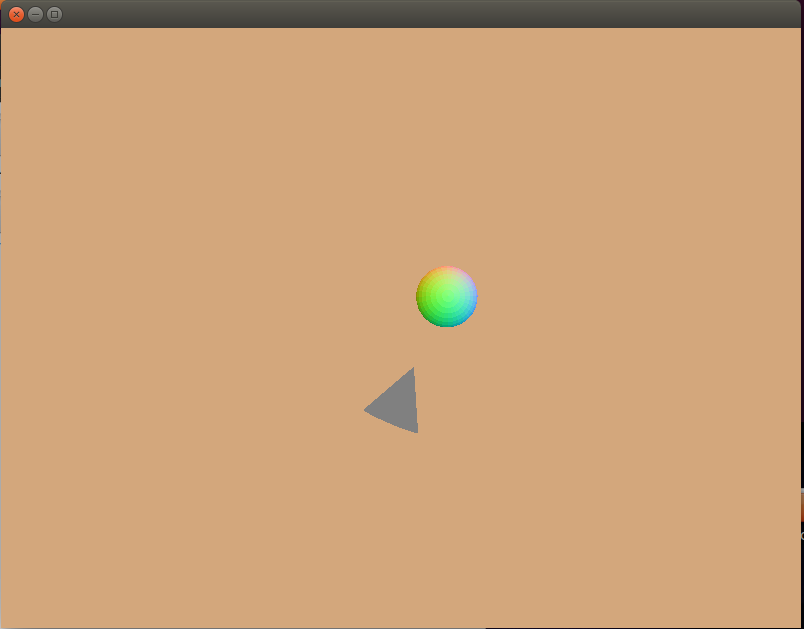
\includegraphics[width=0.5\textwidth]{gameia}
\caption[Programa de prueba 4]{Juego en el que un cono persigue a una esfera controlada por un jugador.}
\label{fig:gameia}
\end{figure}

\begin{figure}[!htbp!]
\centering
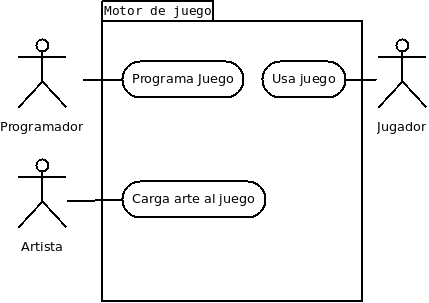
\includegraphics[width=0.8\textwidth]{MCU}
\caption[Diagrama de casos de uso]{}
\label{fig:MCU}
\end{figure}
